% 1 https://quarkus.io 
% 1 https://books.google.at/books?hl=de&lr=&id=AH_EDwAAQBAJ&oi=fnd&pg=PP1&dq=quarkus&ots=ZJfLHasMm9&sig=K7__BsdmoksvoLfJSrqqGOPac1Y&redir_esc=y#v=onepage&q=quarkus&f=false 

\subsection{Allgemeines}
Quarkus wurde kreiert, um Applikationen zu erstellen, welche in einer modernen, Cloud-nativen Welt funktionieren sollen. Quarkus ist ein Kubernetes-natives Java-Framework, auf GraalVM und HotSpot zugeschnitten. Das Ziel von Quarkus ist es, JAVA zur führenden Plattform für Kubernetes und Serverlosen Umgebungen zu machen. Quarkus ist Open Source. 

Die größte Challenge von Mikro Service Architekturen ist, dass die Vermehrung von Services die Komplexität des Systems erhöht. Diese kann mithilfe von Kubernetes-basierenden orchestrierenden Systemen1 gelöst werden, da somit die Effizienz sowie die Ressourcen Verwertung erweitert werden kann. Die Systeme regeln die zeitliche Planung und das Management der Mikro Services in einer dynamischen Weise. Dadurch kann man auch je nach Bedarf an dem System arbeiten, ohne das die Gefahr besteht, dass ein Container ausfällt. Um nun die gesamten Komponenten zusammenzufügen wurde das Framework Quarkus entwickelt. 

Quarkus funktioniert ausgezeichnet, wenn es darum geht Cloud-Native Applikationen von Unternehmen zu managen. Es ist in der Lage kurzen nativen Code aus Java Klassen zu bauen, sowie Container Images daraus zu erstellen. Diese Container können darauffolgend auf Kubernetes laufen. Außerdem unterstützt Quarkus die bekanntesten Java Libraries wie etwa RESTEasy, Hibernate, Apache Kafka, Vert.x, usw. 

Wie nun schon vorher erwähnt, ist eines der vielversprechendsten Features von Quarkus die Fähigkeit aus Applikationen automatisch Container Images zu generieren. Durch das Generieren von Container Images aus nativen Applikationen wird außerdem eine Gefahr zunichte gemacht. Diese hat mit der nativen Ausführung des Programms zu tun, es handelt sich dabei um potentielle Konfliktfehler von Errors, wenn der Build auf einem anderen Operating System stattfand. 
Quarkus sorgt außerdem dafür, Imperative und Reaktive Modelle zu verbinden. Reaktives Programmieren wird immer beliebter, aus dem Grund, dass es in der Lage ist asynchrones Programmieren mit Daten Streams und PROPAGATION OF CHANGE zu verbinden.

\subsection{Architektur}
Im Zentrum von Quarkus liegt die Kern Komponente, welche die Aufgabe hat, die Applikation in der Build-Phase umzuschreiben, um sie perfekt zu optimieren \ref{fig:impl:QuarkusArchitektur}. Daraus entsteht eine native ausführbare und Java-runnable Applikation. Damit der Quarkus Kern diese Arbeit erledigen kann, müssen einige verschiedene Komponenten zusammenarbeiten: 

\begin{compactitem}
    \item Jandex: Ein platzsparender Java Annotation Indexer, sowie eine offline Reflexions Library. Diese Bibliothek ist in der Lage alle runtime sichtbaren Java Annotationen und Klassen Hierarchien für ein Set von Klassen in eine Speicher-effizienten Repräsentation zu indexen.     
    \item Gizmo: Gizmo ist eine Bytecode-Generation Library, welche von Quarkus verwendet wird, um Java Bytecode zu produzieren.             
    \item GraalVM: Ein Set von Komponenten, in welchem jede eine bestimmte Funktion hat. Beispiele dafür sind: ein Compiler, ein SDK API für die Integration von Graal Sprachen und der Konfiguration von native images, runtime Umgebung für JVM-basierte Sprachen
    \item SubstrateVM: Unterkomponente von GraalVM, welches die ahead-of-time (AOT) Kompilation von Java Applikationen von Java Programmen zu eigenständigen ausführbaren Programmen erlaubt.
\end{compactitem}

Des Weiteren gibt es noch einige Quarkus Extensions. Dazu gehören die MicroProfile Spezifikationen, sowie ein Set von Extensions für Hibernate ORM, ein Transaktionsmanager (Narayana), eine Verbindungs-Pool-Manager und viele mehr. 

\begin{figure}[h t]
    \centering
    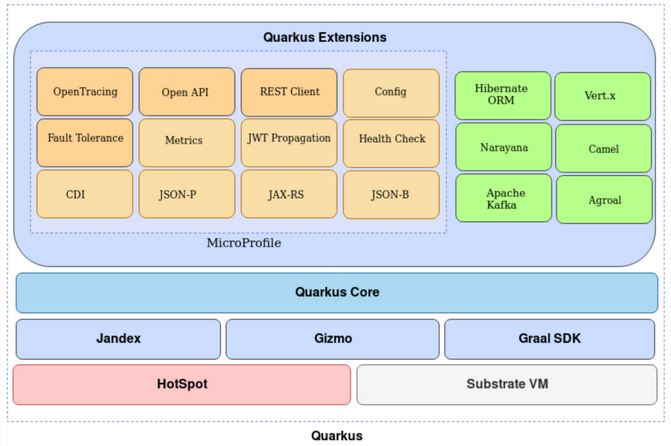
\includegraphics[scale=0.5]{pics/quarkusArchitektur.JPG}
    \caption{Quarkus Architektur}
    \label{fig:impl:QuarkusArchitektur}
\end{figure}

\subsection{Funktionen}
\subsection{Vorteile gegenüber anderen Tools}
\subsection{NodeJS im Vergleich}
\subsection{http GET/POST/PUT Funktionen}
\subsection{JDBC + JPA}